\documentclass[11pt,a4paper]{article}
\usepackage[utf8x]{inputenc}
\title{Lanul de porumb}
\author{Popa Mihai Radu \\Calculatoare Română\\Anul I - Grupa 1.2 B}
\date{Mai 2020}

\usepackage{amsmath}
\usepackage{amsfonts}
\usepackage{url}
\usepackage{hyperref}
\usepackage{caption}
\usepackage{algorithm}
\usepackage[noend]{algpseudocode}
\usepackage{txfonts}
\usepackage{romana}
\usepackage{subcaption}
\usepackage{float}
\usepackage{geometry}
\usepackage[table]{xcolor}
\usepackage{graphicx}
\graphicspath{ {Imagini/} }
\usepackage{romana}
  \geometry{
 a4paper,
 total={200mm,140mm},
 left=35mm,
 right=35mm,
 top=35mm,
 bottom=35mm,
 }

\begin{document}

\begin{titlepage}
    \begin{center}
    \large
    Universitatea din Craiova\\
    Facultatea de Automatică, Calculatoare și Electronică\\
    \vspace{0.5cm}
        
\includegraphics[width=0.3\textwidth]{ace.jpg}
    \vspace{2cm}
    
    \huge{\textbf{\textit{Lanul de porumb}}}
    
    \vspace{1cm}
    
    \large \textbf\\ Popa Mihai Radu\\
    \large{Calculatoare Română}\\
    \large{Anul I}\\
    \large{Grupa 1.2B}\\
    \vfill
    
    \vspace{1cm}
    
    \large
    Mai 2020
    
    \end{center}
    
\end{titlepage}

\section{Enunțul problemei}
 Într-un lan de porumb,cantitatea de porumb ce va putea fi recoltată depinde de distanțele dintre fiecare doi coceni consecutivi aflați pe același rand. Dacă această valoare este mai mică decât o limită minimă prestabilită \emph{d} atunci recolta nu va mai fi optimă deoarece porumbii nu se vor mai putea dezvolta corespunzător. Din acest motiv un agricultor trebuie să elimine o parte din porumbii de pe același rând astfel încat distanța dintre oricare doi coceni succesivi să fie cel puțin \emph{d}. Se consideră că porumbii au fost plantați pe un singur rând. Totodată, agricultorul va trebui să elimine cât mai puțini coceni deoarece prin eliminarea unui cocean producția se va micșora. Se cunosc: i) distanța minimă care trebuie păstrată între oricare doi coceni consecutivi; ii) coordonatele cocenilor plantați pe același rând. Să se determine: i) numărul minim de tulpini care trebuie eliminate astfel încat să se respecte distanța minimă între doi coceni consecutivi; ii) coordonatele cocenilor care trebuie păstrați.
 
\section{Algoritmi}

\begin{algorithm}
\caption*{\textsc{Eliminare-Tulpini(vector, dimensiune, distanta)}}
\begin{algorithmic}[1]
\For{$i \leftarrow 0,dimensiune-1$} 
  \If{$vector[i] = 1$}
   \For{$j \leftarrow i+1,i+distanta-1$}
     \If{$vector[j] = 1$}
      \State $eliminari \leftarrow eliminari + 1$
     \EndIf
     \State $vector[j] \leftarrow 0$
    \EndFor
    \State $i \leftarrow i+distanta-1$
    \State $tulpini\_ramase \leftarrow tulpini\_ramase + 1$
  \EndIf
\EndFor
\If{$vector[dimensiune] = 1$}
 \State $tulpini\_ramase \leftarrow tulpini\_ramase + 1$
\EndIf
\end{algorithmic}
\end{algorithm}

\begin{algorithm}
\caption*{\textsc{Eliminare-Tulpini(vector, dimensiune, distanta)}}
\begin{algorithmic}[1]
\State $eliminari \leftarrow 0$
\State $tulpini\_ramase \leftarrow 0$
\For{$i \leftarrow 0,dimensiune-1$} 
  \If{$vector[i+1]-vector[i] < distanta$}
    \For{$j \leftarrow i+1,dimensiune-1$} 
    \State $vector[j] \leftarrow vector[j+1]$
    \EndFor
    \State $i \leftarrow i-1$
    \State $dimensiune \leftarrow dimensiune-1$
    \State $eliminari \leftarrow eliminari+1$
  \EndIf
\EndFor
\State $aux \leftarrow dimensiune$
\While{$eliminari <= nr\_coordonate$}
    \State $tulpini\_ramase \leftarrow tulpini\_ramase+1$
    \State $eliminari \leftarrow eliminari+1$
\EndWhile
\end{algorithmic}
\end{algorithm}

\clearpage

\subsection{Algoritmul 1}
    \subsubsection{\large Descrierea variabilelor}
    Am folosit contorii i și j pentru a parcurge tabloul unidimensional. Variabila dimensiune reține dimensiunea tabloului unidimensional, variabila tulpini\_ramase reține numărul de tulpini rămase, variabila distanta reține distanța necesară dezvoltării corespunzătoare dintre doi coceni de porumb consecutivi, iar variabila eliminari reține numărul de tulpini eliminate.
    
    \subsubsection{\large Descrierea algoritmului}    
    Algoritmul parcurge cu ajutorul contorului i tabloul unidimensional (lan) completat cu 1 și 0, unde 1 reprezintă existența unei tulpini de porumb, iar 0 lipsa acesteia. Daca pe poziția i se află o tulpină, parcurgem cu ajutorul contorului j tabloul unidimensional până la următoarea tulpină de porumb care respectă distanța minimă necesară dezvoltării corespunzătoare a porumbilor. Daca pe poziția j se află o tulpină, incrementăm numărul de tulpini eliminate. Apoi eliminăm tulpinile parcurse (marcarea cu 0 în tabloul unidimensional). Sărim peste tulpinile parcurse și incrementăm numărul de tulpini rămase cu o unitate. Dacă pe ultima poziție a tabloului unidimensional se află o tulpină de porumb, incrementăm numărul de tulpini rămase cu o unitate.
    
\begin{center}
\begin{tabular}{ c c c c}
 Linie & Cost & Timp de execuție  & Notație asimptotică  \\ 
 1 \\  
 2 & c1 & $\sum\limits_{i=0}^{n-1}c1$ & $O(n)$ \\
 3 \\
 4 & c2 & $\sum\limits_{i=0}^{n-1}\sum\limits_{j=i+1}^{i+n-1}c2$ & $O(n^2)$ \\
 5 & c3 & $\sum\limits_{i=0}^{n-1}\sum\limits_{j=i+1}^{i+n-1}c3$ & $O(n^2)$ \\
 6 & c4 & $\sum\limits_{i=0}^{n-1}\sum\limits_{j=i+1}^{i+n-1}c4$ & $O(n^2)$ \\
 7 & c5 & $\sum\limits_{i=0}^{n-1}c5$ & $O(n)$ \\
 8 & c6 & $\sum\limits_{i=0}^{n-1}c6$ & $O(n)$ \\
 9 & c7 & c7 & $O(1)$ \\
 10 & c8 & c8 & $O(1)$
\end{tabular}
\end{center}

$T(n) = O(n)+O(n^2)+O(n^2)+O(n^2)+O(n)+O(n)+O(1)+O(1)$ \\
$\Longrightarrow T(n)=O(n^2)$ 

Din punct de vedere al timpului de execuție algoritmul are complexitatea $O(n^2)$, iar din punct de vedere al memoriei are complexitatea $O(n)$ sau $O(1)$.

\vspace{5cm}

\subsection{Algoritmul 2}
    \subsubsection{\large Descrierea variabilelor}
    Ceea ce apare în plus față de primul algoritm sunt cele două variabile: aux în care reținem dimensiunea tabloului unidimensional după eliminarea tulpinilor și nr\_coordonate în care reținem numărul de coordonate.
     
    \subsubsection{\large Descrierea algoritmului} 
    Algoritmul parcurge cu ajutorul contorului i tabloul unidimensional (coordonate) sortat strict crescător(cu ajutorul algoritmului quicksort), care stochează coordonatele tulpinilor de porumb. Dacă diferența dintre două coordonate alăturate este strict mai mică decât distanța necesară dezvoltării corespunzătoare a porumbilor se elimină tulpina de pe poziția i+1, deplasând tabloul unidimensional cu o poziție spre stânga. Decrementăm cu o unitate valoarea contorului i pentru a rămâne la poziția curentă. Incrementăm numărul de eliminări cu o unitate și decrementăm dimensiunea tabloului unidimensional cu o unitate deoarece am eliminat o tulpină. Reținem în variabila auxiliară aux dimensiunea tabloului unidimensional după eliminarea tulpinilor. Cu ajutorul instrucțiunii while determinăm numărul de tulpini rămase. \\
\vspace{0,4mm}
    Din punct de vedere al timpului de execuție algoritmul de sortare quicksort are complexitatea $O(n log n)$, iar din punct de vedere al memoriei are complexitatea $O(n)$.
  
\begin{center}
\begin{tabular}{ c c c c}
 Linie & Cost & Timp de execuție  & Notație asimptotică  \\ 
 1 & c1 & c1 & $O(1)$ \\
 2 & c2 & c2 & $O(1)$ \\
 3 \\
 4 & c3 & $\sum\limits_{i=0}^{n-1}c3$ & $O(n)$ \\
 5 \\
 6 & c4 & $\sum\limits_{i=0}^{n-1}\sum\limits_{j=i+1}^{n-1}c4$ & $O(n^2)$ \\
 7 & c5 & $\sum\limits_{i=0}^{n-1}c5$ & $O(n)$ \\
 8 & c6 & $\sum\limits_{i=0}^{n-1}c6$ & $O(n)$ \\
 9 & c7 & $\sum\limits_{i=0}^{n-1}c7$ & $O(n)$ \\
 10 & c8 & c8 & $O(1)$ \\
 11 \\ 
 12 & c9 & $\sum\limits_{eliminari=0}^{nr\_coordonate}c9$ & $O(n)$ \\
 13 & c10 & $\sum\limits_{eliminari=0}^{nr\_coordonate}c10$ & $O(n)$ 
\end{tabular}
\end{center}
    
$T(n) = O(1)+O(1)+O(n)+O(n^2)+O(n)+O(n)+O(n)+O(1)+O(n)+O(n)$ \\
$\Longrightarrow T(n)=O(n^2)$ 
 
Din punct de vedere al timpului de execuție algoritmul are complexitatea $O(n^2)$, iar din punct de vedere al memoriei are complexitatea $O(n)$. \\ 

\begin{center}
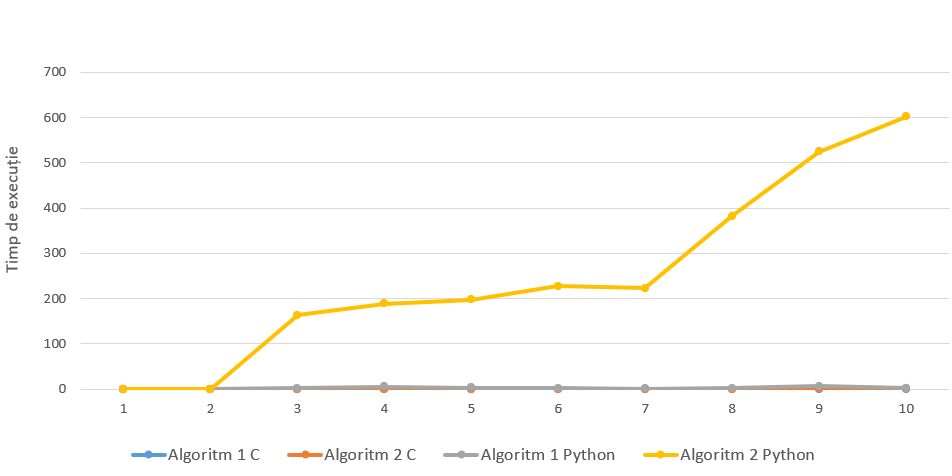
\includegraphics[width=1\textwidth]{diagrama2.png}
\end{center}

\textbf{\textit{Exemple de rulaj:}}

\setlength{\arrayrulewidth}{0.7mm}
\setlength{\tabcolsep}{5pt} 
\renewcommand{\arraystretch}{1}
\definecolor{LightCyan}{rgb}{0.88,1,1}

\begin{table}[h!]
\centering
\begin{tabular}{ |p{13cm}|  }
\hline
\rowcolor{orange} \textbf{Input} \\
\hline
\rowcolor{LightCyan} 10428 3430 \\
\rowcolor{LightCyan} 3648 1159 1706 6936 9796 3112 3101 ... ... ... 4585 1042 399 8382 1321 6526 9085   \\
\hline
\end{tabular}
\end{table}

\vspace*{-\baselineskip}

\setlength{\arrayrulewidth}{0.7mm}
\setlength{\tabcolsep}{5pt}
\renewcommand{\arraystretch}{1}
\definecolor{LightCyan}{rgb}{0.88,1,1}

\begin{table}[h!]
\centering

\begin{tabular}{ |p{13cm}|  }
\hline
\rowcolor{orange} \textbf{Output} \\
\hline
\rowcolor{LightCyan} Numarul minim de tulpini eliminate: 10424 \\ 
\rowcolor{LightCyan} Coordonatele cocenilor ramasi sunt: 0 3430 6860 10290  \\
\rowcolor{LightCyan}  Durata testului: 0.1429999999999s \\
\hline
\end{tabular}
\end{table}     
 
\setlength{\arrayrulewidth}{0.7mm}
\setlength{\tabcolsep}{5pt}
\renewcommand{\arraystretch}{1}
\definecolor{LightCyan}{rgb}{0.88,1,1}

\begin{table}[h!]
\centering
\begin{tabular}{ |p{13cm}|  }
\hline
\rowcolor{orange} \textbf{Input} \\
\hline
\rowcolor{LightCyan} 5 77 \\
\rowcolor{LightCyan} 60 40 13 34 3  \\
\hline
\end{tabular}
\end{table}
   
\vspace*{-\baselineskip}

\setlength{\arrayrulewidth}{0.7mm}
\setlength{\tabcolsep}{5pt}
\renewcommand{\arraystretch}{1}
\definecolor{LightCyan}{rgb}{0.88,1,1}

\begin{table}[h!]
\centering

\begin{tabular}{ |p{13cm}|  }
\hline
\rowcolor{orange} \textbf{Output} \\
\hline
\rowcolor{LightCyan} IMPOSIBIL \\ 
\rowcolor{LightCyan}  Durata testului: 0.0000000000000s \\
\hline
\end{tabular}
\end{table} 
  
\section{Date experimentale}

    Pentru datele experimentale am folosit un algoritm care generează aleatoriu zece seturi de date de intrare, fiecare set având pe prima linie două numere ce reprezintă \emph{numărul de coordonate} și \emph{distanța minimă} care trebuie păstrată între oricare doi coceni consecutivi, iar pe liniile următoare \emph{nr} numere ce reprezintă \emph{coordonatele} cocenilor de porumb.  Parametrul \emph{n} reprezintă limita maximă până la care pot fi generate aleator valori.
    
\begin{algorithm}
\caption*{\textsc{Generator(n)}}
\begin{algorithmic}[1]
\For{$i \leftarrow 1,10$} 
  \State $nr \leftarrow random(1,n)$
  \State $distanta\_minima \leftarrow random(1,n)+1$
  \State $print(nr, distanta\_minima)$
   \For{$j \leftarrow 1,nr$}
    \State $print(random(1,n))$
    \EndFor
\EndFor
\end{algorithmic}
\end{algorithm}    
    
\section{Proiectarea aplicației experimentale}

\subsection{Structura de nivel înalt a aplicației}
  \begin{center}
\begin{tabular}{ c c }
 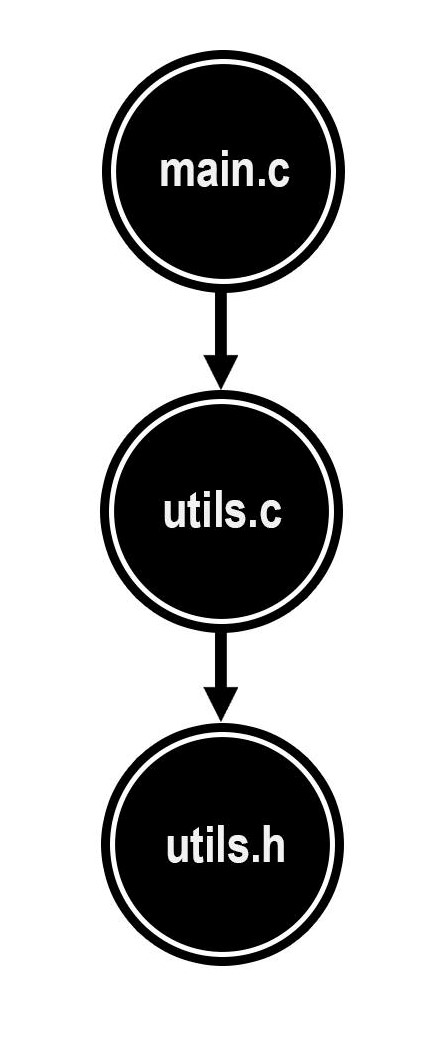
\includegraphics[width=4cm, height=9cm]{algoritm_1.jpg} & 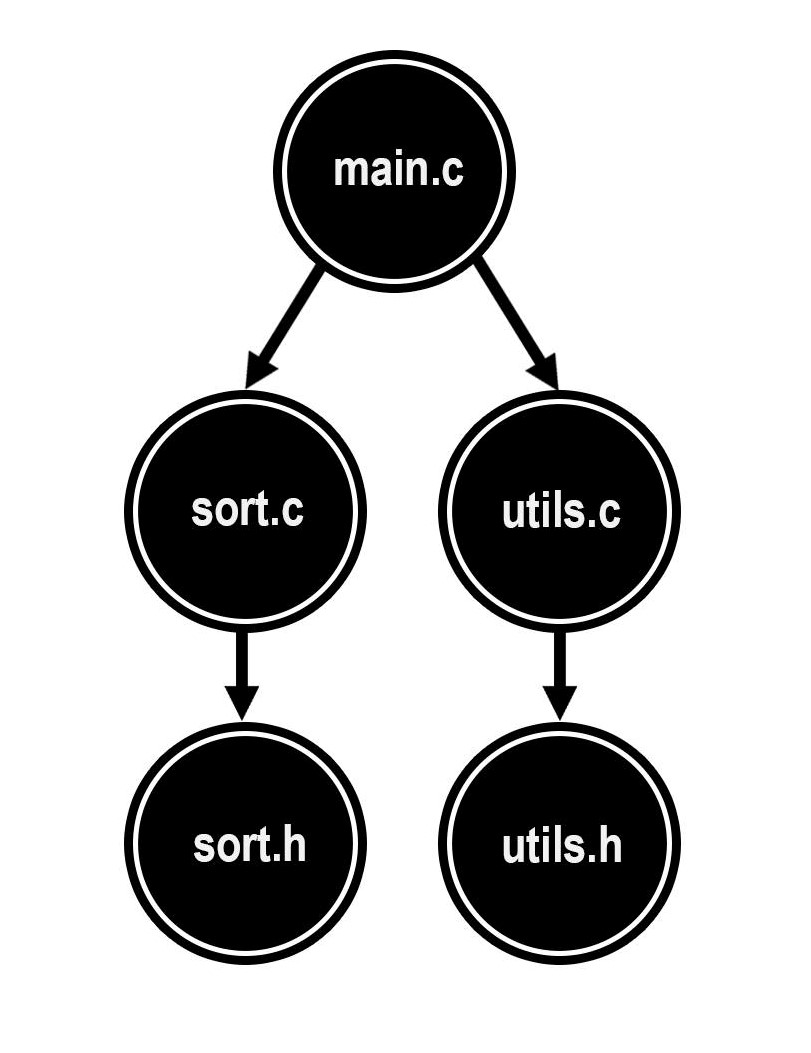
\includegraphics[width=7cm, height=9cm]{algoritm_2.jpg}  \\ 
 Aplicația 1 - Structura pe nivel înalt & Aplicația 2 - Structura pe nivel înalt \\
\end{tabular}
\end{center}
  
  
\subsection{Descrierea mulțimii datelor de intrare}

    Programul citește dintr-un fișier text nr\_coordonate (numărul de coordonate), distanta\_minima (distanța care trebuie păstrată între oricare doi coceni consecutivi) și cele nr\_coordonate (coordonatele cocenilor de porumb).
    
\vspace{0.5cm}

\setlength{\arrayrulewidth}{0.7mm}
\setlength{\tabcolsep}{5pt}
\renewcommand{\arraystretch}{1}
\definecolor{LightCyan}{rgb}{0.88,1,1}

\begin{table}[h!]
\centering
\begin{tabular}{ |p{13cm}|  }
\hline
\rowcolor{orange} \textbf{Input} \\
\hline
\rowcolor{LightCyan} 62 58 \\
\rowcolor{LightCyan} 16 40 54 51 84 61 34 71 53 15 85 0 20 86 80 24 61 34 89 9 69 86 94 46 40 34 6 66 3 45 45 7 32 48 49 78 65 43 88 96 6 25 10 48 66 29 26 4 43 8 93 53 40 36 50 51 76 75 62 72 65 49  \\
\hline
\end{tabular}
\end{table} 

\subsection{Descrierea ieșirilor/rezultatelor}

    Programul afișează într-un fișier text numărul minim de tulpini eliminate, coordonatele cocenilor de porumb rămași și timpul de execuție.
 
\setlength{\arrayrulewidth}{0.7mm}
\setlength{\tabcolsep}{5pt}
\renewcommand{\arraystretch}{1}
\definecolor{LightCyan}{rgb}{0.88,1,1}

\begin{table}[h!]
\centering

\begin{tabular}{ |p{13cm}|  }
\hline
\rowcolor{orange} \textbf{Output} \\
\hline
\rowcolor{LightCyan} Numarul minim de tulpini eliminate: 60 \\ 
\rowcolor{LightCyan} Coordonatele cocenilor ramasi sunt: 0 61 \\
\rowcolor{LightCyan}  Durata testului: 0.0000000000000s \\
\hline
\end{tabular}
\end{table} 
    
    
\subsection{Modulele aplicației}
 
  Aplicația 1 conține următoarele module:
\begin{itemize}
  \item \textbf{\textit{main.c}} - utilizat pentru interfața utilizatorului
  \item \textbf{\textit{utils.c}}, \textbf{\textit{utils.h}} - utilizat pentru funcțiile de generare, afișare și eliminare 
\end{itemize}

\noindent Aplicația 2 conține următoarele module:

\begin{itemize}
  \item \textbf{\textit{main.c}} - utilizat pentru interfața utilizatorului
  \item \textbf{\textit{sort.c}}, \textbf{\textit{sort.h}} - utilizat pentru funcția de sortare și funcțiile auxiliare
  \item \textbf{\textit{utils.c}}, \textbf{\textit{utils.h}} - utilizat pentru funcțiile de generare, afișare și eliminare 
\end{itemize}

\subsection{Funcțiile aplicației}

    \emph{Aplicația 1}
\begin{itemize}
    \item \textbf{\textit{utils.c}} conține următoarele funcții: 
    \begin{enumerate}
        \item \textbf{\textit{generator}} - generează aleatoriu datele de intrare  \\
        Funcția conține un singur parametru \emph{n} ce reprezintă limita maximă până la care pot fi generate aleator valori.
        \item \textbf{\textit{afisare\_coordonate}} - afișează coordonatele cocenilor de porumb rămași \\
        Funcția conține doi parametri: \emph{vector} și \emph{dimensiune}. Parametrul \emph{vector} este o mulțime de valori care reprezintă lanul de porumb, iar parametrul \emph{dimensiune} reprezintă numărul de elemente ale mulțimii.
        \item \textbf{\textit{eliminare\_tulpini}} - elimină tulpinile de porumb care nu respectă distanța minimă \\
        Funcția conține trei parametri: \emph{vector}, \emph{dimensiune}, \emph{distanta}. Parametrul \emph{vector} este o mulțime de valori care reprezintă lanul de porumb, parametrul \emph{dimensiune} reprezintă numărul de elemente ale mulțimii, iar parametrul \emph{distanta} reprezintă distanța minimă ce trebuie păstrată între doi coceni consecutivi.
    \end{enumerate}
\end{itemize} 
 
\vspace{4cm}  

\noindent \emph{Aplicația 2}
\begin{itemize}
    \item \textbf{\textit{sort.c}} conține următoarele funcții: 
     \begin{enumerate}
        \item \textbf{\textit{interchange\_values}} - interschimbă două elemente  \\
        Funcția conține doi parametri: \emph{address\_1} si \emph{address\_2}.
        Parametrul \emph{address\_1} este un pointer la adresa primului element, iar parametrul \emph{address\_2} este un pointer la adresa celui de-al doilea element.
        \item \textbf{\textit{partition}} - ia ultimul element ca pivot, plasează
        elementul pivot pe poziția sa corectă în vectorul sortat, toate elementele mai mici decât pivotul la stânga pivotului, iar toate elementele mai mari la dreapta pivotului \\
        Funcția conține trei parametri: \emph{vector}, \emph{left} și \emph{right}.  Parametrul \emph{vector} reprezintă un pointer la mulțimea de valori care urmează să fie sortată, parametrul \emph{left} reprezintă indexul de pornire, iar parametrul \emph{right} reprezintă imdexul de oprire.
        \item \textbf{\textit{quick\_sort}} - funcția principală ce implementează quicksort \\
         Funcția conține trei parametri: \emph{vector}, \emph{left} și \emph{right}. Parametrul \emph{vector} reprezintă un pointer la mulțimea de valori care urmează să fie sortată, parametrul \emph{left} reprezintă indexul de pornire, iar parametrul \emph{right} reprezintă imdexul de oprire.
    \end{enumerate}
    
    \item \textbf{\textit{utils.c}} conține următoarele funcții: 
    \begin{enumerate}
        \item \textbf{\textit{generator}} - generează aleatoriu datele de intrare  \\
        Funcția conține un singur parametru \emph{n} ce reprezintă numărul maxim până la care pot fi generate aleator valori.
        \item \textbf{\textit{afisare\_coordonate}} - afișează coordonatele cocenilor de porumb rămași \\
        Funcția conține doi parametri: \emph{vector} și \emph{dimensiune}. Parametrul \emph{vector} este o mulțime de valori care reprezintă coordonatele cocenilor de porumb, iar parametrul \emph{dimensiune} reprezintă numărul de elemente ale mulțimii.
        \item \textbf{\textit{eliminare\_tulpini}} - elimină tulpinile de porumb care nu respectă distanța minimă \\
        Funcția conține trei parametri: \emph{vector}, \emph{dimensiune}, \emph{distanta}. Parametrul \emph{vector} este o mulțime de valori care reprezintă coordonatele cocenilor de porumb, parametrul \emph{dimensiune} reprezintă numărul de elemente ale mulțimii, iar parametrul \emph{distanta} reprezintă distanța minimă ce trebuie păstrată între doi coceni consecutivi.
    \end{enumerate}
    
\end{itemize}    

\section{Rezultate \& concluzii}
    \subsection{Rezultate}
    Mai jos se poate observa o analiză comparativă a timpilor de execuție obținuți în urma rulării celor doi algoritmi implementați. Se observă faptul că algoritmul 1 este mai eficient decât algoritmul 2. Limbajul C este mult mai rapid decât limbajul Python, deoarece Python este un limbaj interpretat, iar C este un limbaj compilat. \\

\begin{center}
  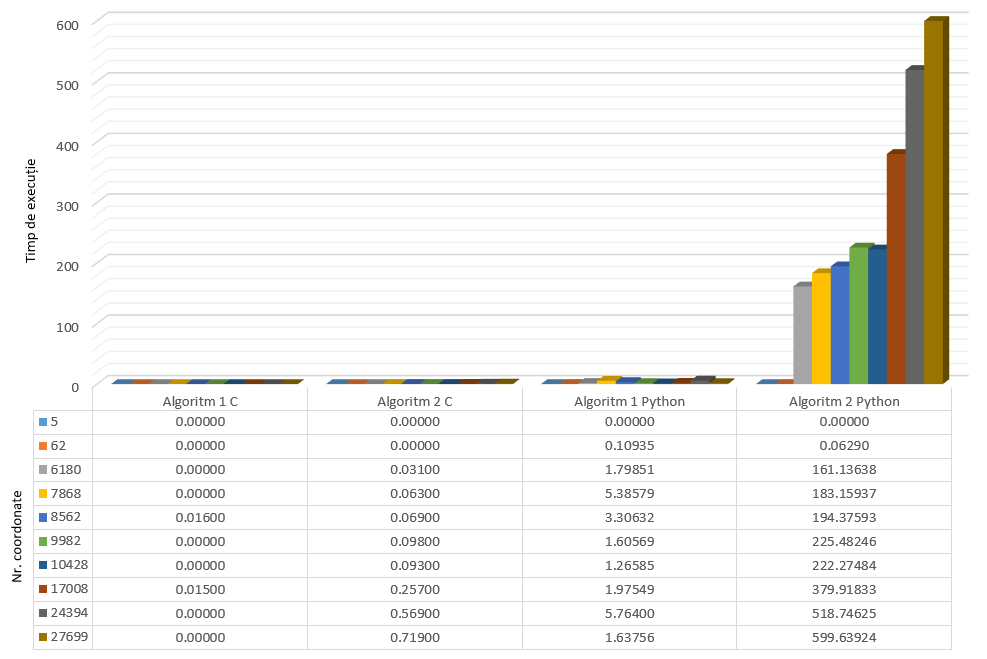
\includegraphics[width=1\textwidth]{diagrama1.png} \\
\end{center}

    \subsection{Concluzii}
    Când am început să scriu codul pentru acest proiect , obiectivul meu principal a fost să-l scriu cât de simplu se poate. Aceasta a fost probabil cea mai provocatoare parte a proiectului. După terminarea acestuia pot spune că am învățat că uneori este mai important cum găsești rezultatul decât rezultatul în sine. Acest proiect a fost foarte interesant pentru mine. Ca direcții viitoare, voi  încerca să reduc numărul de caractere pe care le oferă programul, astfel încât acesta să poată rula mai repede.

\begin{thebibliography}{9}

    \bibitem{cormen09}
	  Thomas H. Cormen and Charles E. Leiserson and Ronald L. Rivest and Clifford Stein,
	  \emph{Introduction to Algorithms}.
	  MIT Press,
	  3rd Edition,
	  2009.

     \bibitem{python}
     w3schools -- 
      \url{https://www.w3schools.com/python/}, 
     accesat în Aprilie 2020.
     
     \bibitem{latex}
     overleaf --
     \url{https://www.overleaf.com/learn/latex/Main_Page},
     accesat în Aprilie 2020.
     
     \bibitem{latex2}
     wikibooks --
     \url{https://en.wikibooks.org/wiki/LaTeX/Algorithms}, 
     accesat în Aprilie 2020.
     
     \bibitem{latex3}
     stackexchange --
     \url{https://tex.stackexchange.com/},
     accesat în Aprilie 2020
     
\end{thebibliography}

\end{document}
